%%%%%%%%%%%%%%%%%%%%%%%%%%%%%%%%%%%%%%%%%%%%%%%%%%%%%%%%%%%%%%%%%%
%%	  mmm  mmmmmm mm   m        m    m mmmmmm  mmmm				%%
%%	m"   " #      #"m  #        #    # #      #    #			%%
%%	#   mm #mmmmm # #m #        #    # #mmmmm "mmmm"			%%
%%	#    # #      #  # #  """   #    # #      	   #			%%
%%	 "mmm" #mmmmm #   ##        "mmmm" #mmmmm  #mmm"			%%
%%							      								%%
%%                                                              %%
%%                                                              %%
%%      Grundlagen der Elektrischen Netzwerke, UE               %%
%%      Gruppe 5, Team F                                        %%
%%      Authors: Severin Wolf, Maximilian Seidler.              %%
%%%%%%%%%%%%%%%%%%%%%%%%%%%%%%%%%%%%%%%%%%%%%%%%%%%%%%%%%%%%%%%%%%

\documentclass[a4paper]{article}

\usepackage{pstricks}
\usepackage{pst-circ}
\usepackage{pst-plot}
\usepackage{pstricks-add}
\usepackage[ngerman, english]{babel} 
\usepackage{amsmath}
\usepackage[latin1]{inputenc}
\usepackage{geometry}
\geometry{a4paper,left=3cm,right=2cm, top=2cm, bottom=2cm} 
\usepackage{graphicx}
\usepackage[EFvoltages, european, straightvoltages]{circuitikz}

\newpsobject{showgrid}{psgrid}{subgriddiv=1,griddots=10,gridlabels=0pt}
\psset{unit=1.0cm}
\psset{tensioncolor=blue}
\psset{tensionlabelcolor=blue}
\psset{intensitycolor=red}
\psset{intensitylabelcolor=red}

\setlength{\parindent}{0pt}
\usepackage{lipsum}

\newcommand\blfootnote[1]{%
	\begingroup
	\renewcommand\thefootnote{}\footnote{#1}%
	\addtocounter{footnote}{-1}%
	\endgroup
}
\begin{document}
	\pagestyle{empty} \enlargethispage*{25cm}\samepage{
		
		\vspace*{-3cm}
		\begin{center}
			\begin{minipage}[!h]{18cm}
				\hspace*{-0.9cm}
				\includegraphics[width=3.3cm]{./Figures/igte_logo}
				\begin{tabular}{p{10cm}}
					\vspace{1cm}
					\centering{
						\Large Institute of Fundamentals and Theory in
						Electrical Engineering\\
						Graz University of Technology\\
						~\\
						~\\}
				\end{tabular}
				\includegraphics[width=3.3cm]{./Figures/TUG_logo}
			\end{minipage}
			
			\vspace*{0.5cm}
			\Large
			\textbf{Fundamentals of electical circuits} \\
			\textbf{9. Homework}\\
			Multiports
			\vspace*{0.5cm}
			
			\large
			27 May 2021
	\end{center}}
	
	\vspace*{0.2cm}
	
	%%%%%%%%%%%%%%%%%%%%%%%%%%%%%%%%%%%%%%%%%%%%%%%%%%%%%%%%%%%%%%%%%%%%
	%%%%%%%%%%%%%%%%%%%%%%%%%%%%%%%%%%%%%%%%%%%%%%%%%%%%%%%%%%%%%%%%%%%%
	
	Consider the given circuit in figure~\ref{circuit}. There are three two-ports with passive elements connected in a cascade.

	\begin{enumerate}
		\item Determine the \textbf{Z}- and the \textbf{Y} set of parameters (independendly of each other), if possible. If it's not possible to calculate one of the parameter-sets, explain the reason briefly. Double-check your results by using the parameter conversion table ($[\underline{Z}] \rightarrow [\underline{Y}]$).
		
		\item Find the \textbf{A}-parameters (ABCD matrix) by using the parameter conversion table for all three two-port circuits.

		\item Calculate the voltage transfer-function $H(s) = \frac{U_{out}(s)}{U_{in}(s)}$ of the complete cascade connection. Bring the transfer-function in the following form: $H(s) = K\cdot \frac{s^2}{(1+\frac{s}{\omega_1})(1+\frac{s}{\omega_2})}$. Calculate the values of $K$, $\omega_1$ and $\omega_2$.

		\item Confirm the expression for the transfer-function in Matlab. \\
		Construct a Bode amplitude and phase-angle plot of the total transfer-function. 
		
		\item Simulate the circuit in LT-SPICE and compare the results for the transfer-function $H(s) = \frac{U_{out}(s)}{U_{in}(s)}$. 
	\end{enumerate}

	\subsection*{Values:}
$R_1=50~\Omega $, $R_2=2~k\Omega$, $R_3=600~\Omega$, $C=400 \mu F$, $L=20mH$.
\vspace{0.5cm}\\
\textbf{\textbf{Hint:} }
useful Matlab commands: \textbf{zpk, minreal, bode, zpkdata}.
 	
 	\begin{figure}[h!]
 		\centering
 		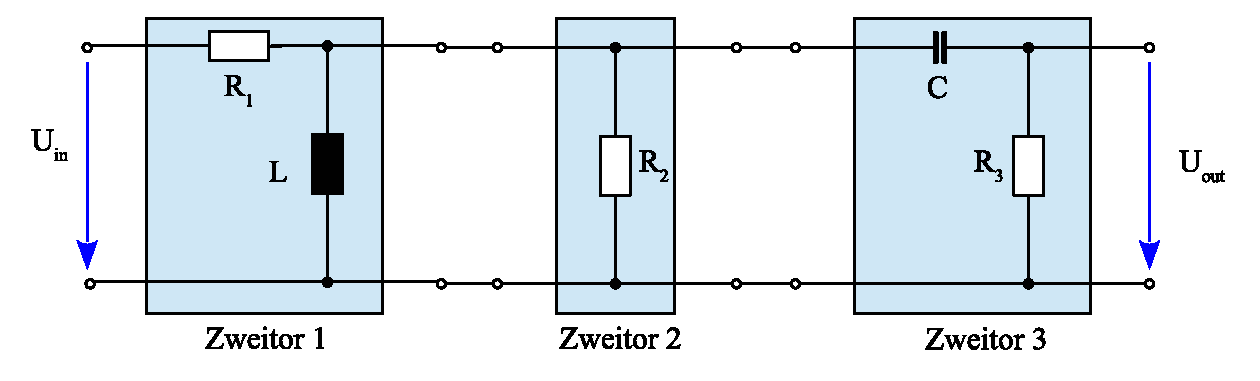
\includegraphics[width=1\textwidth]{./Figures/homework9_circuit.eps}
 		\caption{Teil 1 - cascade connection of three two-ports}
 		\label{circuit}
 	\end{figure}
\vspace{3.5cm}
 	\blfootnote{Deadline: 10 June 2021; \qquad Team I}

\pagebreak

\section{Solution}
\subsection{Determination of the Z-Matrix}
Two-port 1:
\begin{figure}[!h] \centering
	\begin{circuitikz}
		\draw(0,0)
		to[short, o-*](4,0)
		to[short, -o](5,0);
		\draw(0,5)
		to[short, o-](0.5,5)
		to[short, i=$\underline{I_1}$, color=red](1,5)
		to[R,l=$R_1$](3,5)
		to[short,-*](4,5)
		to[short, i<=$\underline{I_2}$, color=red](5,5)
		to[short,-o](5,5);
		\draw(4,0)
		to[short](4,1)
		to[L, l=$L$](4,4)
		to[short, i<=$\underline{I_1} + \underline{I_2}$, color=red](4,5);
		\draw[-{Latex[length=2mm]}, color=blue] (0, 4.5) -- (0, 0.5)
	  	node[pos=0.5, left] {$\underline{U_{in}}$};
		\draw[-{Latex[length=2mm]}, color=blue] (5, 4.5) -- (5, 0.5)
	  	node[pos=0.5, right] {$\underline{U_{out}}$};
	\end{circuitikz}	
\end{figure}
\\
\begin{equation*}
	\begin{bmatrix}
		\underline{U_{in}}\\ \underline{U_{out}}\\
	\end{bmatrix} =
	\begin{bmatrix}
		\underline{Z_{11}} & \underline{Z_{12}}\\
		\underline{Z_{21}} & \underline{Z_{22}}\\
	\end{bmatrix} \cdot
	\begin{bmatrix}
		\underline{I_{1}}\\ \underline{I_{2}}\\
	\end{bmatrix}\\
\end{equation*}
\begin{align*}
	M1&: \underline{U_{in}} = R_1 \cdot \underline{I_1} + j\omega L \cdot(\underline{I_1} + \underline{I_2}) =
	\underline{I_1} \cdot (R_1 + j\omega L) + \underline{I_2} \cdot j\omega L
	\\
	M2&: \underline{U_{out}} = j\omega L \cdot(\underline{I_1} + \underline{I_2}) =
	\underline{I_1} \cdot j\omega L + \underline{I_2} \cdot j\omega L
\end{align*}
With these two mesh equations we could determine our impedances and set up the Z-Matrix.
\begin{equation*}
	\begin{bmatrix}
		\underline{Z}
	\end{bmatrix}=
	\begin{bmatrix}
		R_1 + j\omega L & j\omega L\\
		j\omega L & j\omega L\\
	\end{bmatrix}
\end{equation*}

Two-port 2:
\begin{figure}[!h] \centering
	\begin{circuitikz}
		\draw(0,0)
		to[short, o-*](2.5,0)
		to[short, -o](5,0);
		\draw(0,5)
		to[short, o-](0.5,5)
		to[short, i=$\underline{I_1}$, color=red](1,5)
		to[short,-*](2.5,5)
		to[short, i<=$\underline{I_2}$, color=red](5,5)
		to[short,-o](5,5);
		\draw(2.5,0)
		to[short](2.5,1)
		to[R, l=$R_2
		$](2.5,4)
		to[short, i<=$\underline{I_1} + \underline{I_2}$, color=red](2.5,5);
		\draw[-{Latex[length=2mm]}, color=blue] (0, 4.5) -- (0, 0.5)
	  	node[pos=0.5, left] {$\underline{U_{in}}$};
		\draw[-{Latex[length=2mm]}, color=blue] (5, 4.5) -- (5, 0.5)
	  	node[pos=0.5, right] {$\underline{U_{out}}$};
	\end{circuitikz}	
\end{figure}
\\
\begin{equation*}
	\begin{bmatrix}
		\underline{U_{in}}\\ \underline{U_{out}}\\
	\end{bmatrix} =
	\begin{bmatrix}
		\underline{Z_{11}} & \underline{Z_{12}}\\
		\underline{Z_{21}} & \underline{Z_{22}}\\
	\end{bmatrix} \cdot
	\begin{bmatrix}
		\underline{I_{1}}\\ \underline{I_{2}}\\
	\end{bmatrix}\\
\end{equation*}
\begin{align*}
	M1&: \underline{U_{in}} = R_2 \cdot(\underline{I_1} + \underline{I_2}) =
	\underline{I_1} \cdot R_2 + \underline{I_2} \cdot R_2
	\\
	M2&: \underline{U_{out}} = R_2 \cdot(\underline{I_1} + \underline{I_2}) =
	\underline{I_1} \cdot R_2 + \underline{I_2} \cdot R_2
\end{align*}
With these two mesh equations we could determine our impedances and set up the Z-Matrix.
\begin{equation*}
	\begin{bmatrix}
		\underline{Z}
	\end{bmatrix}=
	\begin{bmatrix}
		R_2 & R_2\\
		R_2 & R_2\\
	\end{bmatrix}
\end{equation*}

\pagebreak

Two-port 3:
\begin{figure}[!h] \centering
	\begin{circuitikz}
		\draw(0,0)
		to[short, o-*](4,0)
		to[short, -o](5,0);
		\draw(0,5)
		to[short, o-](0.5,5)
		to[short, i=$\underline{I_1}$, color=red](1,5)
		to[C,l=$C$](3,5)
		to[short,-*](4,5)
		to[short, i<=$\underline{I_2}$, color=red](5,5)
		to[short,-o](5,5);
		\draw(4,0)
		to[short](4,1)
		to[R, l=$R_3$](4,4)
		to[short, i<=$\underline{I_1} + \underline{I_2}$, color=red](4,5);
		\draw[-{Latex[length=2mm]}, color=blue] (0, 4.5) -- (0, 0.5)
	  	node[pos=0.5, left] {$\underline{U_{in}}$};
		\draw[-{Latex[length=2mm]}, color=blue] (5, 4.5) -- (5, 0.5)
	  	node[pos=0.5, right] {$\underline{U_{out}}$};
	\end{circuitikz}	
\end{figure}
\\
\begin{equation*}
	\begin{bmatrix}
		\underline{U_{in}}\\ \underline{U_{out}}\\
	\end{bmatrix} =
	\begin{bmatrix}
		\underline{Z_{11}} & \underline{Z_{12}}\\
		\underline{Z_{21}} & \underline{Z_{22}}\\
	\end{bmatrix} \cdot
	\begin{bmatrix}
		\underline{I_{1}}\\ \underline{I_{2}}\\
	\end{bmatrix}\\
\end{equation*}
\begin{align*}
	M1&: \underline{U_{in}} = \frac{1}{j\omega C} \cdot \underline{I_1} + R_3 \cdot(\underline{I_1} + \underline{I_2}) =
	\underline{I_1} \cdot \left(\frac{1}{j\omega C} + R_3 \right) + \underline{I_2} \cdot R_3
	\\
	M2&: \underline{U_{out}} = R_3 \cdot(\underline{I_1} + \underline{I_2}) =
	\underline{I_1} \cdot R_3 + \underline{I_2} \cdot R_3
\end{align*}
With these two mesh equations we could determine our impedances and set up the Z-Matrix.
\begin{equation*}
	\begin{bmatrix}
		\underline{Z}
	\end{bmatrix}=
	\begin{bmatrix}
		\frac{1}{j\omega C} + R_3 & R_3\\
		R_3 & R_3\\
	\end{bmatrix}
\end{equation*}

\subsection{Determination of the Y-Matrix}

\begin{equation*}
	\begin{bmatrix}
		\underline{I_1}\\ \underline{I_2}\\
	\end{bmatrix} =
	\begin{bmatrix}
		\underline{Y_{11}} & \underline{Y_{12}}\\
		\underline{Y_{21}} & \underline{Y_{22}}\\
	\end{bmatrix} \cdot
	\begin{bmatrix}
		\underline{U_{in}}\\ \underline{U_{out}}\\
	\end{bmatrix}\\
\end{equation*}
We determine the Y-matrix using the node-voltage-method:\\
Two-port 1:
\begin{equation*}
	\begin{bmatrix}
		\underline{Y}
	\end{bmatrix}=
	\begin{bmatrix}
		\frac{1}{R_1} & -\frac{1}{R_1}\\
		-\frac{1}{R_1} & \frac{1}{R_1} + \frac{1}{j\omega L}\\
	\end{bmatrix}
\end{equation*}
We check this result with the conversion table\\\\
\begin{tabular}{c|c|c|c|c|c|c}
	$\underline{Z}$ & 1 & $\underline{Z_{11}}$ & $\underline{Z_{12}}$ & $\underline{Z_{21}}$ & $\underline{Z_{22}}$ & $det[\underline{Z}]$\\[1ex]
	\hline 
	$\underline{Y}$ & $det[\underline{Y}]$ & $\underline{Y_{22}}$ & $-\underline{Y_{12}}$ & $-\underline{Y_{21}}$ & $\underline{Y_{11}}$ & 1\\[1ex]
\end{tabular}\\\\

\begin{equation*}
	det[\underline{Z}] = (R_1 + j\omega L) \cdot j\omega L - (j\omega L)^2 = R_1 \cdot j\omega L
\end{equation*}
and we see, our calculations are correct.\\
\\
Two-port 2:\\
For this two-port the Y-matrix does not exist.
\begin{equation*}
	det[\underline{Z}] = R_2^2 - R_2^2 = 0
\end{equation*}
This is, because the determinant of it's Z-matrix is zero.
Because of this, we would have to divide by zero in order to calculate X, which is not possible.

Two-port 3:
\begin{equation*}
	\begin{bmatrix}
		\underline{Y}
	\end{bmatrix}=
	\begin{bmatrix}
		j\omega C & -j\omega C\\
		-j\omega C & j\omega C + \frac{1}{R_3}\\
	\end{bmatrix}
\end{equation*}

We check this result with the conversion table\\\\
\begin{tabular}{c|c|c|c|c|c|c}
	$\underline{Z}$ & 1 & $\underline{Z_{11}}$ & $\underline{Z_{12}}$ & $\underline{Z_{21}}$ & $\underline{Z_{22}}$ & $det[\underline{Z}]$\\[1ex]
	\hline 
	$\underline{Y}$ & $det[\underline{Y}]$ & $\underline{Y_{22}}$ & $-\underline{Y_{12}}$ & $-\underline{Y_{21}}$ & $\underline{Y_{11}}$ & 1\\[1ex]
\end{tabular}\\\\

\begin{equation*}
	det[\underline{Z}] = (\frac{1}{j\omega C} + R_3) \cdot R_3 - R_3^2 = \frac{1}{j\omega C} \cdot R_3
\end{equation*}
\\
and we see, our calculations are correct.\\

\subsection*{Determination of the A-Matrix}
In order to calculate the transfer function we need to determine the A-matrix. We do this with the following parameter
conversion table:\\\\
\begin{tabular}{|c|c|c|c|c|c|c|}
	\hline
	$\underline{Z}$ & 1 & $\underline{Z_{11}}$ & $\underline{Z_{12}}$ & $\underline{Z_{21}}$ & $\underline{Z_{22}}$ & $det[\underline{Z}]$\\[1ex]
	\hline 
	$\underline{Y}$ & $det[\underline{Y}]$ & $\underline{Y_{22}}$ & $-\underline{Y_{12}}$ & $-\underline{Y_{21}}$ & $\underline{Y_{11}}$ & 1\\[1ex]
	\hline
	$\underline{A}$ & $\underline{A_{21}}$ & $\underline{A_{11}}$ & $det[\underline{A}]$ & 1 & $\underline{A_{22}}$ &$\underline{A_{12}}$\\[1ex]
	\hline
\end{tabular}\\\\
Two-port 1:\\
\begin{equation*}
	\begin{bmatrix}
		\underline{A}
	\end{bmatrix}=
	\frac{1}{j\omega L} \cdot
	\begin{bmatrix}
		R_1 + j\omega L & R_1 \cdot j\omega L\\
		1 & j\omega L\\
	\end{bmatrix} =
	\begin{bmatrix}
		\frac{R_1}{j\omega L} + 1 & R_1\\
		\frac{1}{j\omega L} & 1\\
	\end{bmatrix}
\end{equation*}

Two-port 2:\\
\begin{equation*}
	\begin{bmatrix}
		\underline{A}
	\end{bmatrix}=
	\frac{1}{R_2} \cdot
	\begin{bmatrix}
		R_2 & 0\\
		1 & R_2\\
	\end{bmatrix} =
	\begin{bmatrix}
		1 & 0\\
		\frac{1}{R_2} & 1\\
	\end{bmatrix}
\end{equation*}

Two-port 3:\\
\begin{equation*}
	\begin{bmatrix}
		\underline{A}
	\end{bmatrix}=
	\frac{1}{R_3} \cdot
	\begin{bmatrix}
		\frac{1}{j\omega C} + R_3 & \frac{1}{j\omega C} \cdot R_3\\
		1 & R_3\\
	\end{bmatrix} =
	\begin{bmatrix}
		\frac{1}{j\omega C \cdot R_3} + 1 & \frac{1}{j\omega C}\\
		\frac{1}{R_3} & 1\\
	\end{bmatrix}
\end{equation*}

Now that we have the A-matrices of the three parts, we can calculate the A-matrix for the whole
cascade. We do this by multiplicating the three A-matrices.

\begin{equation*}
	\begin{bmatrix}
		\underline{A}
	\end{bmatrix}=
	\begin{bmatrix}
		\underline{A_1}
	\end{bmatrix}\cdot
	\begin{bmatrix}
		\underline{A_2}
	\end{bmatrix}\cdot
	\begin{bmatrix}
		\underline{A_3}
	\end{bmatrix}
\end{equation*}
\begin{equation*}
	\begin{bmatrix}
		\underline{A}
	\end{bmatrix}=
	\begin{bmatrix}
		\frac{R_1}{j\omega L} + 1 & R_1\\
		\frac{1}{j\omega L} & 1\\
	\end{bmatrix}\cdot
	\begin{bmatrix}
		1 & 0\\
		\frac{1}{R_2} & 1\\
	\end{bmatrix}\cdot
	\begin{bmatrix}
		\frac{1}{j\omega C \cdot R_3} + 1 & \frac{1}{j\omega C}\\
		\frac{1}{R_3} & 1\\
	\end{bmatrix}
\end{equation*}
\begin{equation*}
	\begin{bmatrix}
		\underline{A}
	\end{bmatrix}=
	\begin{bmatrix}
		\frac{R_1}{j\omega L} + \frac{R_1}{R_2} + 1 & R_1\\
		\frac{1}{j\omega L} + \frac{1}{R_2} & 1\\
	\end{bmatrix}\cdot
	\begin{bmatrix}
		\frac{1}{j\omega C \cdot R_3} + 1 & \frac{1}{j\omega C}\\
		\frac{1}{R_3} & 1\\
	\end{bmatrix}
\end{equation*}
\begin{equation*}
	\begin{bmatrix}
		\underline{A}
	\end{bmatrix}=
	\begin{bmatrix}
		\left(\frac{R_1}{j\omega L} + \frac{R_1}{R_2} + 1\right)\left(\frac{1}{j\omega C \cdot R_3} + 1\right) + \frac{R_1}{R_3} &
		\left(\frac{R_1}{j\omega L} + \frac{R_1}{R_2} + 1\right)\frac{1}{j\omega C} + R_1\\
		\left(\frac{1}{j\omega L} + \frac{1}{R_2}\right)\left(\frac{1}{j\omega C \cdot R_3} + 1\right) + \frac{1}{R_3} &
		\left(\frac{1}{j\omega L} + \frac{1}{R_2}\right)\frac{1}{j\omega L} + 1
	\end{bmatrix}
\end{equation*}

\pagebreak

\subsection{Calculating the Transfer Function}
In order to make calculations easier we substitue $j\omega$ with $s$
\begin{equation*}
	\underline{H(s)} = \frac{\underline{U_{out}(s)}}{\underline{U_{in}(s)}} = \frac{1}{\underline{A_{11}}}
\end{equation*}
\begin{align*}
	\underline{A_{11}} &= \left(\frac{R_1}{sL} + \frac{R_1}{R_2} + 1\right)\left(\frac{1}{sC \cdot R_3} + 1\right) + \frac{R_1}{R_3}\\
	\underline{A_{11}} &= \frac{R_1}{s^2LCR_3} + \frac{R_1}{sL} + \frac{R_1}{sCR_2R_3} + \frac{R_1}{R_2} + \frac{1}{sCR_3} + 1 + \frac{R_1}{R_3}\\
	\underline{A_{11}} &= \frac{R_1R_2 + R_1sCR_3R_2 + R_1sL + R_1s^2LCR_3 + sLR_2 + s^2LCR_3R_2}{s^2LCR_3R_2}\\
	\underline{A_{11}} &= \frac{s^2(R_1LCR_3 + LCR_3R_2 + R_1LCR_2) + s(R_1CR_3R_2 + R_1L + LR_2) + R_1R_2}{s^2LCR_3R_2}\\
	\underline{H(s)} &= \frac{1}{\underline{A_{11}}} = \frac{s^2LCR_3R_2}{s^2(R_1LCR_3 + LCR_3R_2 + R_1LCR_2) + s(R_1CR_3R_2 + R_1L + LR_2) + R_1R_2}\\
	\underline{H(s)} &= \frac{s^2}{s^2\left( \frac{R_1}{R_2} + \frac{R_1}{R_3} + 1 \right) + s\left( \frac{R_1}{L} + \frac{R_1}{CR_3R_2} + \frac{1}{CR_3} \right) + \frac{R_1}{LCR_3}}\\
\end{align*}
For the next step we need to factorise the denominator. In order to do that we use the following substitutions:
\begin{align*}
	a &= \frac{R_1}{R_2} + \frac{R_1}{R_3} + 1\\
	b &= \frac{R_1}{L} + \frac{R_1}{CR_3R_2} + \frac{1}{CR_3}\\
	c &= \frac{R_1}{LCR_3}\\
\end{align*}
Now we can calculate the zeropoints:
\begin{align*}
	s_1 & = \frac{-b + \sqrt{b^2 - 4ac}}{2a}\\
	s_2 & = \frac{-b - \sqrt{b^2 - 4ac}}{2a}\\
\end{align*}
Finally we can factorise the denominator:
\begin{align*}
	\underline{H(s)} &= \frac{s^2}{(s-s_1)(s-s_2)} = \frac{s^2}{-s_1\left(1 + \frac{s}{-s_1}\right) \cdot -s_2\left(1 + \frac{s}{-s_2}\right)} =
	\frac{1}{s_1s_2} \cdot \frac{s^2}{\left(1 + \frac{s}{-s_1}\right) \left(1 + \frac{s}{-s_2}\right)}
\end{align*}
With that we have reached the form:
\begin{equation*}
	\underline{H(s)} = K\cdot \frac{s^2}{\left(1+\frac{s}{\omega_1}\right)\left(1+\frac{s}{\omega_2}\right)}
\end{equation*}
with
\begin{align*}
	\omega_1 &= -s_1 = -\frac{-b + \sqrt{b^2 - 4ac}}{2a}\\
	\omega_2 &= -s_2 = -\frac{-b - \sqrt{b^2 - 4ac}}{2a}\\
	K &= \frac{1}{s_1s_2} = \frac{1}{\frac{-b + \sqrt{b^2 - 4ac}}{2a} \cdot \frac{-b - \sqrt{b^2 - 4ac}}{2a}}\\
\end{align*}
\end{document}